\documentclass[a4paper]{article}

%% Language and font encodings
%\usepackage{fontspec}
%\setmainfont{Times New Roman}\usepackage{CormorantGaramond}
\usepackage[toc,page]{appendix}
\usepackage[T1]{fontenc}
\usepackage[utf8x]{inputenc}
\usepackage[swedish, english]{babel}
\usepackage{float}
\usepackage[colorlinks=true, allcolors=black]{hyperref}
\usepackage[dvipsnames]{xcolor}
\usepackage{tikz}
\usepackage{circuitikz} % for circuit diagrams
\usepackage{caption}
\usepackage{subcaption}
\usepackage{graphicx}
\usepackage{mathtools}
\urlstyle{tt}
\newcommand{\email}[1]{\href{mailto:#1}{\tt{\nolinkurl{#1}}}}
\newcommand{\orcid}[1]{ORCID: \href{https://orcid.org/#1}{\tt{\nolinkurl{#1}}}}

\usepackage[parfill]{parskip}
\renewcommand*\oldstylenums[1]{\carlitoOsF #1}
% \usepackage{fancyhdr}
%\usepackage{natbib}
\usepackage{authblk}
\setlength{\headheight}{41pt}
\setlength{\textwidth}{440pt}
%\pagestyle{fancy}

%% Sets page size and margins
\usepackage[a4paper,top=3cm,bottom=2cm,left=3cm,right=3cm,marginparwidth=1.75cm]{geometry}

%% Useful packages
\usepackage{graphicx}
\usepackage{booktabs}
%\usepackage{caption}
\usepackage{amsmath}
\usepackage{mathtools}

\usepackage{titlesec}
\setcounter{secnumdepth}{4}

\usepackage[colorinlistoftodos]{todonotes}
\usepackage[yyyymmdd]{datetime}
\renewcommand{\dateseparator}{-}
\rmfamily
% \fancyhead[L]{\rmfamily Bi-MMC battery}

\def\fc{\textit{f\textsubscript{c}}} % carrier frequency 
\def\fo{\textit{f\textsubscript{o}}} % reference frequency 

% \usepackage[utf8]{inputenc}

%% Package to import MATLAB codes
\usepackage{listings}
%\usepackage[usenames,dvipsnames]{color}

% This is the color used for MATLAB comments below
%\definecolor{MyDarkGreen}{rgb}{0.0,0.4,0.0}

% For faster processing, load Matlab syntax for listings
%\lstloadlanguages{Matlab}%
\definecolor{codegreen}{rgb}{0,0.6,0}
\definecolor{codegray}{rgb}{0.5,0.5,0.5}
\definecolor{codepurple}{rgb}{0.58,0,0.82}
\definecolor{mygreen}{RGB}{28,172,0} 
\definecolor{mylilas}{RGB}{170,55,241}
\definecolor{backcolour}{rgb}{0.95,0.95,0.92}
	
\lstdefinestyle{mystyle}{
	backgroundcolor=\color{backcolour},   
	commentstyle=\color{codegreen},
	keywordstyle=\color{blue},
	numberstyle=\tiny\color{codegray},
	stringstyle=\color{codepurple},
	basicstyle=\ttfamily\scriptsize,
	breakatwhitespace=false,         
	breaklines=true,                 
	captionpos=b,                    
	keepspaces=true,                 
	numbers=left,                    
	numbersep=5pt,                  
	showspaces=false,                
	showstringspaces=false,
	showtabs=false,                  
	tabsize=2,
	aboveskip=\medskipamount
}
\lstset{style=mystyle,language=MATLAB}

%\lstset{ 
%	language=Matlab,                		% choose the language of the code
%	%	basicstyle=10pt,       				% the size of the fonts that are used for the code
%	numbers=left,                  			% where to put the line-numbers
%	numberstyle=\footnotesize,      		% the size of the fonts that are used for the line-numbers
%	stepnumber=1,                   			% the step between two line-numbers. If it's 1 each line will be numbered
%	numbersep=5pt,                  		% how far the line-numbers are from the code
%	%	backgroundcolor=\color{white},  	% choose the background color. You must add \usepackage{color}
%	showspaces=true,               		% show spaces adding particular underscores
%	showstringspaces=true,         		% underline spaces within strings
%	showtabs=true,                 			% show tabs within strings adding particular underscores
%	%	frame=single,	                			% adds a frame around the code
%	%	tabsize=2,                				% sets default tabsize to 2 spaces
%	%	captionpos=b,                   			% sets the caption-position to bottom
%	breaklines=true,                			% sets automatic line breaking
%	breakatwhitespace=false,        		% sets if automatic breaks should only happen at whitespace
%	escapeinside={\%*}{*)}          		% if you want to add a comment within your code
%}

\title{\Large PhD course in simulation: DAE exercises}
\author{Arvind Balachandran}
\date{\today}

\begin{document}
	
	\maketitle
	\pagenumbering{gobble}
	\newpage
	\pagenumbering{arabic}
	\section*{Uppgift 2.1}
	\begin{enumerate}
	\item[(a)] Determine differential index for the differential equation.
	\begin{equation*}
		y' = u
	\end{equation*}
\end{enumerate}

Differential index : 0

\fbox{\begin{minipage}[h!]{\textwidth}
		No need to differentiate the above expression to reduce it to an ODE (or) you differentiate the above equation 0 times to reduce it to an ODE. Therefore, index 0
\end{minipage}}

\begin{enumerate}
	\item[(b)] Determine differential index for the differential equation.
	\begin{align*}
		e_1: \dot x = u,\\
		e_2: y = x.
	\end{align*}
\end{enumerate}

From $e_1$ and $e_2$ it is clear that $x$ and $y$ are dynamic variables. Therefore, it is clear that we need to differentiate $e_2$ to get $\dot y$. This makes the differential index as 2.
	\pagebreak
	\section*{Uppgift 2.2}
	Consider the following DAE:
\begin{equation*}
	\begin{pmatrix}
		0 & 0\\
		1 & \eta\,t 
	\end{pmatrix} \, \begin{pmatrix}
		\dot x \\
		\dot y
	\end{pmatrix} + 
	\begin{pmatrix}
		1 & \eta\,t \\
		0 & 1 + \eta
	\end{pmatrix} \,
	\begin{pmatrix}
		x \\
		y
	\end{pmatrix} =
	\begin{pmatrix}
		q \\
		0
	\end{pmatrix}
\end{equation*}
with $\eta$ > −1 and where $q$ is an arbitrary function of $t$.

\begin{enumerate}
	\item[(a)] DAE has differential index 2 \\
	We have,
	\begin{align*}
		e_1\,:\,x + \eta\,t\,y &= q, & e_2\,:\,\dot x + \eta\,t\,\dot y + \left(1 + \eta\right)\,y &= 0,
	\end{align*}
	where $x$, $y$ are dynamic variables. In order to achive an ODE of the form $\dot X = f(X,t)$, where $X$ is the dynamic variable. We differentiate $e_1$:
	\begin{align*}
		\dot e_1\,:\,\dot x + \eta\,t\,\dot y + \eta\,y &= \dot q, & e_2\,:\,\dot x &= -\eta\,t\,\dot y - \left(1 + \eta\right)\,y.
	\end{align*}
	Furthermore, we substitute $e_2$ in $\dot e_1$. Thus we get:
	\begin{align*}
		\dot e_1\,: -y &= \dot q, & e_2\,:\,\dot x &= -\eta\,t\,\dot y - \left(1 + \eta\right)\,y.
	\end{align*}
	Now $e_2$ is not of the form $\dot X = f(X,t)$. Therefore, we differentiate $ \dot e_1 $. We get:
	\begin{align*}
		\ddot e_1\,: -\dot y &= \ddot q, & e_2\,:\,\dot x &= -\eta\,t\,\ddot q - \left(1 + \eta\right)\,y.
	\end{align*}
	\fbox{\begin{minipage}[h!]{\textwidth}
			Here we differentiated the algebraic equation twice to reduce the above set of equations to an explicit ODE. Therefore the differential index is 2.
	\end{minipage}}\\
	\item[(b)] Exact solution \\
	We know that from $\dot e_1$ that $y = -\dot q$ is one solution. Now integrating $e_2$ we get, $ x = \eta\,t\,\dot q + q $.
	\item[(c)] Assuming that there is a new solution to the problem:
	\begin{align*}
		e_1\,:\tilde y &= -\dot q + f_1 & e_2\,:\tilde x &= \eta\,t\,\dot q + q + f_2,
	\end{align*}
	where $f_1$ and $f_2$ are arbitrary functions. 
	
	Substitution in the original DAE system, we get:
	\begin{align*}
		e_3\,:\,\tilde x + \eta\,t\,\tilde y &= q, & e_4\,:\,\dot{\tilde x} + \eta\,t\,\dot{\tilde y} + \left(1 + \eta\right)\,\tilde y &= 0.
	\end{align*}
	Considering $e_3$:
	\begin{align*}
		\eta\,t\,\dot q + q + f_2 - \eta\,t\,\dot q + \eta\,t\,f_1 &= q & \implies f_2 + \eta\,t\,f_1 &= 0 \quad :\,e_3
	\end{align*}
	Considering $e_4$:	
	\begin{align*}
		\eta\,t\,\ddot q + \eta\,\dot q + \dot q + \dot f_2 + \eta\,t\,(-\ddot q + \dot f_1) + \left(1 + \eta\right)\,(-\dot q + f_1) &= 0, \\
		\eta\,t\,\ddot q + \eta\,\dot q + \dot q + \dot f_2 - \eta\,t\,\ddot q + \eta\,t\,\dot f_1 - \dot q - \eta\,\dot q + f_1 + \eta\,f_1 &= 0\\
		\dot f_2 + \eta\,t\,\dot f_1 + \left(1 + \eta\right)\,f_1 &= 0\,:\,e_5.
%		\eta\,t\,\ddot q + \dot q + \dot f_2 - \eta\,t\,\ddot q + \eta\,t\,\dot f_1 - \dot q + f_1 - \eta\,\dot q + \eta\,f_1 &= 0 & \implies \dot f_2 + \eta\,t\,\dot f_1 + f_1 - \eta\,\dot q + \eta\,f_1 &= 0 \,:\,e_4
	\end{align*}	
	From $e_3$, we know $f_2 + \eta\,t\,f_1 = 0 $. Therefore, $\dot f_2 + \eta\,t\,\dot f_1 = 0 $. Thus, $e_5$ becomes:
	\begin{align*}
		f_1\,\left(1+\eta\right) &= 0
	\end{align*}
	\fbox{\begin{minipage}[h!]{\textwidth}
		For $\eta \neq -1$, $f_1 = 0$, from $e_3$, $f_2 = 0$. Therefore, $y = -\dot q$ and $ x = \eta\,t\,\dot q + q $ are the only solutions to the ODE.
	\end{minipage}}\\
	\item[(d)] Applying backward Euler to (a), we get: 
	\begin{align*}
		x_n + \eta\,t_n\,y_n &= q_n & \frac{x_n - x_{n-1}}{h} + \eta\,t_n\,\frac{y_n - y_{n-1}}{h} + y_n + \eta\,y_n &= 0.
	\end{align*}
	Substituting the left equation in the right equation, we get:
	\begin{align*}
		\frac{q_n - \eta\,t_n\,y_n - x_{n-1}}{h} + \eta\,t_n\,\frac{y_n - y_{n-1}}{h} + y_n + \eta\,y_n &= 0
	\end{align*}
	Thus,
	\begin{align*}
		y_n = \frac{1}{h\,\left(1 + \eta\right)}\,\left(x_{n-1} + \eta\,t_n\,y_{n-1} - q_n\right).
	\end{align*}
	The error in $y$ can be written as follows:
	\begin{align*}
		e^y_n = y(t) - y_n = y(t) - \frac{1}{h\,\left(1 + \eta\right)}\,\left(x_{n-1} + \eta\,t_n\,y_{n-1} - q_n\right)
	\end{align*}
	Substituting $y(t) = -\dot q$ and $x_n = q_{n-1} - \eta\,t_{n-1}\,y_{n-1}$, we get:
	\begin{align*}
		e^y_n = - \dot q - \frac{1}{h\,\left(1 + \eta\right)}\,\left(q_{n-1} - \eta\,t_{n-1}\,y_{n-1} + \eta\,t_n\,y_{n-1} - q_n\right).
	\end{align*}
	We know that, $h = t_n - t_{n-1}$. Therefore, 
	\begin{align*}
		e^y_n = - \dot q - \frac{1}{h\,\left(1 + \eta\right)}\,\left(q_{n-1} + \eta\,h\,y_{n-1} - q_n\right) = -\dot q - \frac{1}{\left(1 + \eta\right)}\left(\eta\,y_{n-1} - \frac{q_n - q_{n-1}}{h}\right).
	\end{align*}	
	We also know that, $\dot q = \frac{q_n - q_{n-1}}{h} + O(h)$. So,
	\begin{align*}
		e^y_n = -\dot q - \frac{1}{\left(1 + \eta\right)}\left(\eta\,y_{n-1} - \dot q + O(h)\right).
	\end{align*}
	We also need the error in the previous step, i.e, $e^y_{n-1} = y(t_{n-1}) - y_{n-1}$ Thus,
	\begin{align*}
		e^y_n = -\dot q - \frac{1}{\left(1 + \eta\right)}\left(\eta\,\left(y(t_{n-1}) - e^y_{n-1}\right) - \dot q + O(h)\right).
	\end{align*}
%	Assuming that the difference method is consistent (or accurate) of order $p$, i.e,
%	\begin{align*}
%		\textbf{d}_n &= O(h), & \implies & \frac{y(t_n) - y(t_{n-1})}{h} - f(t_{n-1},y_{n-1}) = O(h), \\
%		\implies \frac{y(t_n) - y(t_{n-1})}{h} - y(t_{n-1}) &= O(h), & \implies & \dot q_n - \left(\dot q_{n-1} + h\,y_{n-1}\right) = h\,O(h), 
%	\end{align*}
%	\begin{align*}
%		\frac{y(t-n)}{}
%	\end{align*}
	\textbf{Do not know how to proceed from here!}
\end{enumerate}


%\begin{enumerate}
%	\item[(c)] Exact solution 
%\end{enumerate}
	\pagebreak
	\section*{Uppgift 2.3}
	Jian helped! 

The index 3 DAE is given as follows:
\begin{align*}
	x &= g(t) & \implies x &= g\\
	\dot x - y &= 0 & \implies y &= \dot g\\
	\dot y - z &= 0 & \implies z &= \ddot g\\
\end{align*}
Assuming that $\frac{h_{n-1}}{h_n}$ is not $\infty$, then $\mathcal{O}(h_{n}\,h_{n-1}) = \mathcal{O}(h_n^2)$. 

From the DAE system we have:
\begin{align*}
	y_n &= \frac{g_n - g_{n-1}}{h_n},\\
	y_{n-1} &= \frac{g_{n-1} - g_{n-2}}{h_{n-1}},\\
	z_n &= \frac{y_n - y_{n-1}}{h_n},\\
\end{align*}
Now, 
\begin{align*}
	g_{n-1} &= g_n - \dot g_n\,h_n + \frac{1}{2}\,h_n^2\,\ddot g_n + \mathcal{O}(h_n^3),\\
	g_{n-2} &= g_n - \dot g_n\,\left(h_n + h_{n-1}\right) + \frac{1}{2}\,\left(h_n + h_{n-1}\right)^2\,\ddot g_n + \mathcal{O}(h_n^3)
\end{align*}
Thus, 
\begin{align*}
	z_n &= \frac{y_n - y_{n-1}}{h_n} = \frac{\frac{g_n - g_{n-1}}{h_n} - \frac{g_{n-1} - g_{n-2}}{h_{n-1}}}{h_n} =  \frac{1}{2}\,\left(1+\frac{h_{n-1}}{h_n}\right)\,\ddot g + \mathcal{O}(h_n)
\end{align*}
The error is,
\begin{align*}
	z_n - \ddot g_n = \frac{1}{2}\,\left(\frac{h_{n-1}}{h_n} - 1 \right)\,\ddot g + \mathcal{O}(h_n)
\end{align*}

	\pagebreak
	\section*{Uppgift 2.7}
	\begin{enumerate}
	\item[(a)] Consistent initial condition on $ x(0),\,\dot x(0),\,\ddot x(0)\,\dots $ for
	\begin{align*}
		E_1\,&:\,\begin{cases} 
			\dot x &= x + y,\\
			0 &= x + 2y + a(t).
		\end{cases} & 
		E_2\,&:\,\begin{cases} 
			\dot x_1 &= -x_1 + x_2 + a(t),\\ 
			\dot x_2 &= -x_2 + x_3 + b(t),\\ 	
			0 &= x_2 + c(t).
		\end{cases} 
	\end{align*}
	Considering $E_1$ we have the dynamic state $ x $ and the algebraic variable $ y $. We need an initial condition for $x(0),\ \&\ y(0)$. $ y(0) $ is chosen arbitrarily but $x$ is constrained by the equation: $x = - \left(2y + a(t)\right)$.\\
	Considering $E_2$ we have the dynamic states $ x_1,\,x_2 $ and the algebraic variable $ x_3 $. Differentiating $ E_2(3) $, we get:
	\begin{align*}
		\begin{cases} 
			E_2(1)\,:\,\dot x_1 &= -x_1 + x_2 + a(t),\\ 
			E_2(2)\,:\,\dot x_2 &= -x_2 + x_3 + b(t),\\ 	
			\dot E_2(3)\,:\dot x_2 &= -\dot c(t).
		\end{cases} 
	\end{align*}
	From this it is clear that $ x_2(0) = \dot c(0) + b(0) + x_3(0),\ x_2(0) = -c(0)  $, this constraints $ x_2,\ x_3 $. However, there are not constrains on $ x_1 $.\\
	\item[(b)] Hidden constrains
	\begin{align*}
		\dot x_1 + x_3 &= f_1 \\
		\dot x_2 + x_1 &= f_2 \\
		x_2 &= f_3. 
	\end{align*}
	\item[(c)] Differential index calculation.
	\begin{align*}
		e_1:\dot x_1 + \dot x_2 &= u_1,\\
		e_2:x_1 - x_2 &= u_2.
	\end{align*}
	Differentiation $ e_2 $,
	\begin{align*}
		e_1:\dot x_1 + \dot x_2 &= u_1,\\
		\dot e_2:\dot x_1 - \dot x_2 &= \dot u_2.
	\end{align*}
	Substituting $ e_1 $ and $ \dot e_2 $,
	\begin{align*}
		e_1:\dot x_1 &= \frac{u_1 + \dot u_2}{2},\\
		\dot e_2:2\dot x_2 &= u_1 - \dot u_2 .
	\end{align*}
	Therefore, the differential index is 1.\\
	\item[(d)] Differential index
	\begin{align*}
		e_1:\dot x_1 + x_3 &= u_1,\\
		e_2:x_1 - x_2 &= u_2,\\
		e_3:\dot x_2 = x_3.
	\end{align*}
	Differentiating $ e_2 $,
	\begin{align*}
		e_1:\dot x_1 + x_3 &= u_1,\\
		\dot e_2:\dot x_1 - x_3 &= \dot u_2,\\
		e_3:\dot x_2 = x_3.
	\end{align*}
	Differentiating $ \dot e_2 $,
		\begin{align*}
		e_1:\dot x_1 &= u_1 - x_3 ,\\
		\ddot e_2:2\,\dot x_3 &=  \dot u_1 - \ddot u_2,\\
		e_3:\dot x_2 = x_3.
	\end{align*}
	The differential index in now 2 for the same set of equations but with the addition of a variable.
\end{enumerate}
	\pagebreak
	\section*{Uppgift 2.9}
	\subsection*{(a) General DAE}
\begin{equation*}
	F(\dot x, x, \theta) = 0,\ x(0) = x_0(\theta)
\end{equation*}

Derive a differential equation for 
\begin{equation*}
	P (t) = \frac{dx(t)}{d\theta} = x_\theta
\end{equation*}

differentiating the first equation with respect to $\theta$, we get:
\begin{align*}
	\frac{dF}{d\theta} &= F_{\dot x}\,{\dot x}_\theta + F_{x}\,{x}_\theta + F_{\theta} = 0
%	\dot x_\theta &= -F_{\dot x}^{-1}\,F_{x}\,{x}_\theta - F_{\dot x}^{-1}\,F_{\theta}
\end{align*}
\subsection*{ (b) Semi-explicit DAE}
\begin{equation*}
	\dot x = F(x, y, \theta),\ x(0) = x_0(\theta), 0 = H(x,y,\theta)
\end{equation*}
differentiating the first equation with respect to $\theta$, we get:
\begin{align*}
	\dot x_p &= F_x\,x_p + F_y\,y_p + F_\theta & 0 = H_x\,x_p + H_y\,y_p + H_p
\end{align*}
\fbox{\begin{minipage}[h!]{\textwidth}
The equations for the sensitivity functions in both cases are rather similar except for the general ODE, we have the mass matrix that has to be taken into consideration. 
\end{minipage}}
\subsection*{(c) Implement sensitivity analysis for a DAE}
Reproducing the results in Section 4.3 (Figs 7-16) in the paper Timothy Maly, Linda R. Petzold, \textit{Numerical methods and software for sensitivity analysis of differential-algebraic systems}
\begin{figure}[h!b!]
	\centering
	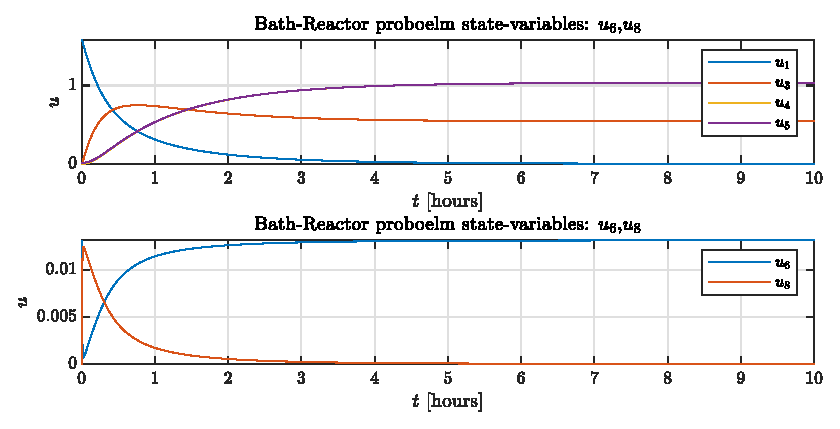
\includegraphics[width=\textwidth]{Figures/Ugf2_9c1.eps}
\end{figure}

The code for reproducing the results 
\begin{lstlisting}
%%% the initial conditions
p = [21.8893;... p1(0)
	2.14e9;... p2(0)
	32.318;... p3(0)
	21.893;... p4(0)
	1.07e9;... p5(0)
	7.65e-18;... p6(0)
	4.03e-11;... p7(0)
	5.32e-18;... p8(0)
	];
%%% the parameters
uo1 = 1.5776;
u7 = 0.5*(p(7) + sqrt(p(7)^2 + 4*p(7)*uo1)); u8 = u7;
u0 = [uo1 8.32 0 0 0 0.0131 u7 u8 0 0];


%%% the batch reactor problem
batch_reactor = @(t,u) [...
	-p(3)*u(2)*u(8)											  ;...u1'
	-p(1)*u(2)*u(6) + p(2)*u(10)     - p(3)*u(2)*u(8)         ;... u2'
	p(3)*u(2)*u(8) + p(4)*u(4)*u(6) - p(5)*u(9)               ;... u3'
	-p(4)*u(4)*u(6) + p(5)*u(9)                               ;... u4'
	p(1)*u(2)*u(6) - p(2)*u(10)                               ;... u5'
	-p(1)*u(2)*u(6) - p(4)*u(4)*u(6) + p(2)*u(10) + p(5)*u(9) ;... u6'
	-0.0131 + u(6) + u(8) + u(9) + u(10)                      ;... u7'    
	u(8)  - p(7)*u(1)/(p(7) + u(7))                           ;... u8
	u(9)  - p(8)*u(3)/(p(8) + u(7))                           ;... u9
	u(10) - p(6)*u(5)/(p(6) + u(7))                           ;... u10
];

%%% the mass matrix
M = diag([ones([1,7]) 0 0 0]);

%%% the simualtion ------------
ts = linspace(0,10,10000); % step-time of 0.001 s
options = odeset('Mass',M); % the mass matrix
[tsim,usim] = ode15s(@(t,y) batch_reactor(t,y),ts,u0,options); % BDF implicit solver
\end{lstlisting}

The Sensitivity analysis goes as follows, the code does not work but I am not sure as to why that is happening.
\begin{lstlisting}
	%% the sensitivity analysis
	% using symbolic toolbox to find out all the derivatives
	
	% clear all% temp
	
	params = sym('p',[1 8]); % parameters 
	u_syms = sym('u',[10 1]); % parameters 
	f_syms = [...
	-params(3)*u_syms(2)*u_syms(8); ...u1'
	-params(1)*u_syms(2)*u_syms(6) + params(2)*u_syms(10)     - params(3)*u_syms(2)*u_syms(8)         ;... u2'
	params(3)*u_syms(2)*u_syms(8) + params(4)*u_syms(4)*u_syms(6) - params(5)*u_syms(9)              ;... u3'
	-params(4)*u_syms(4)*u_syms(6) + params(5)*u_syms(9)                               ;... u4'
	params(1)*u_syms(2)*u_syms(6) - params(2)*u_syms(10)                              ;... u5'
	-params(1)*u_syms(2)*u_syms(6) - params(4)*u_syms(4)*u_syms(6) + params(2)*u_syms(10) + params(5)*u_syms(9) ;... u6'
	-0.0131 + u_syms(6) + u_syms(8) + u_syms(9) + u_syms(10)                      ;... u7'    
	u_syms(8)  - params(7)*u_syms(1)/(params(7) + u_syms(7))                           ;... u8
	u_syms(9)  - params(8)*u_syms(3)/(params(8) + u_syms(7))                           ;... u9
	u_syms(10) - params(6)*u_syms(5)/(params(6) + u_syms(7))                           ;... u10
	];% f_syms(t) = u_syms'(t)
	
	fp_syms = [diff(f_syms,params(1)),...
	diff(f_syms,params(2)),...
	diff(f_syms,params(3)),...
	diff(f_syms,params(4)),...
	diff(f_syms,params(5)),...
	diff(f_syms,params(6)),...
	diff(f_syms,params(7)),...
	diff(f_syms,params(8))
	]; % fp
	
	fx_syms = [diff(f_syms,u_syms(1)),...
	diff(f_syms,u_syms(2)),...
	diff(f_syms,u_syms(3)),...
	diff(f_syms,u_syms(4)),...
	diff(f_syms,u_syms(5)),...
	diff(f_syms,u_syms(6)),...
	diff(f_syms,u_syms(7)),...
	diff(f_syms,u_syms(8)),...
	diff(f_syms,u_syms(9)),...
	diff(f_syms,u_syms(10))
	]; % fx
	
	f = matlabFunction(f_syms,'Vars',[{u_syms} {params}]);
	fp = matlabFunction(fp_syms,'Vars',[{u_syms} {params}]);
	fx = matlabFunction(fx_syms,'Vars',[{u_syms} {params}]);
	
	% Xp' = Fx*Xp + Fp
	Xp0 = zeros(10,8); % initital condition
	
	Fsens = @(t,Xp) fx(interp1(tsim,usim,t,'spline')',p').*squeeze(Xp)' + fp(interp1(tsim,usim,t,'spline')',p');
	
	[tsens,Psens] = ode15s(@(t,y) Fsens(t,y),ts,Xp0);
\end{lstlisting}

	\pagebreak
	\section*{Uppgift 2.10}
	\begin{enumerate}
	\item[(a)] \textit{Differential index of the model? }
	
	Considering no grounding point, we get:
	\begin{align*}
		C\,\left((v_1 - v_2)' - (v_3 - v_2)'\right) &= i;  & e_1\\
		-C\,\left((v_1 - v_2)' - (v_3 - v_2)'\right) + \frac{1}{R}\,(v_3 - v_2) &= 0;  & e_2\\
		v_1 - v_2 &= v(t);  & e_3.
	\end{align*}
	
	Considering ground point 2. By simplifying and differentiating $e_3$, we get:
	\begin{align*}
		v_3' &= \frac{1}{R\,C}\,v_3 + \frac{1}{C}\,v'(t); & e_2\\
		v_1' &= v'(t); & e_3'
	\end{align*}

	\fbox{\begin{minipage}[h!]{\textwidth}
				Therefore, the differential index is 1. 
	\end{minipage}}

	\textit{Does it matter for the index if the grounding point instead had been in point 1 or 3?} 
	
	Considering ground point 2. By simplifying and differentiating $e_3$, we get:
	\begin{align*}
		v_3' &= \frac{1}{R\,C}\,v_3 + \frac{1}{C}\,v'(t); & e_2\\
		v_2' &= -v'(t); & e_3'
	\end{align*}

	\fbox{\begin{minipage}[h!]{\textwidth}
		Therefore, the differential index is 1. 
	\end{minipage}}

	Considering ground point 3. By simplifying and differentiating $e_3$, we get:
	\begin{align*}
		v_1' &= -\frac{1}{R\,C}\,v_1 + \frac{1}{C}\,v'(t); & e_2\\
		v_2' &= -v'(t); & e_3'
	\end{align*}
	
	\fbox{\begin{minipage}[h!]{\textwidth}
			Therefore, the differential index is 1. 
	\end{minipage}}
	The differential index does not change by changing the grounding point.	

	\item[(b)] What is the structural index for the model?
	
	Considering ground point 2, we get:
	\begin{center}
		\begin{tabular}{c|c c c}
			& $v_1'$ & $v_3'$ & i \\
			\hline
			$e_1$ & X & X & X \\
			$e_2$ & X & X &  \\
			$e_3$ &  &  &  \\
		\end{tabular} $\underrightarrow{\text{differentiating}\,e_3}$
	\begin{tabular}{c|c c c}
		& $v_1'$ & $v_3'$ & i \\
		\hline
		$e_1$ & X & X & \textbf{X} \\
		$e_2$ & X & \textbf{X} &  \\
		$e_3'$ & \textbf{X} &  &  \\
	\end{tabular} 
	\end{center}

	\fbox{\begin{minipage}[h!]{\textwidth}
		The matrix now has full rank. The structural index is 2 (1+1). 
	\end{minipage}}
	
	\item[(c)] What is the structural index for the model if the grounding point had been
	in point 1 or 3?
	
	Considering ground point 1, we get:
	\begin{center}
		\begin{tabular}{c|c c c}
			& $v_2'$ & $v_3'$ & i \\
			\hline
			$e_1$ & & X & X \\
			$e_2$ & & X &  \\
			$e_3$ & & &  \\
		\end{tabular} $\underrightarrow{\text{differentiating}\,e_3}$
	\begin{tabular}{c|c c c}
		& $v_2'$ & $v_3'$ & i \\
		\hline
		$e_1$ & & X & \textbf{X} \\
		$e_2$ & & \textbf{X} &  \\
		$e_3'$ & \textbf{X} & &  \\
	\end{tabular}
	\end{center}
	
	\fbox{\begin{minipage}[h!]{\textwidth}
			The matrix now has full rank. The structural index is 2 (1+1). 
	\end{minipage}}
	
	Considering ground point 3, we get:
	\begin{center}
		\begin{tabular}{c|c c c}
			& $v_1'$ & $v_2$ & i \\
			\hline
			$e_1$ & X &  & \textbf{X} \\
			$e_2$ & X & \textbf{X} &  \\
			$e_3$ & \textbf{X} & X &  \\
		\end{tabular} 
	\end{center}
	
	\fbox{\begin{minipage}[h!]{\textwidth}
			The matrix now has full rank. The structural index is 1 (0+1). 
	\end{minipage}}
	
	\item[(d)]  Index and the structural index for the model
	\textit{Differential index}
	\begin{align*}
		\dot x + \dot y + x + y &= \cos(t) & e_1\\
		\dot x + \dot y + x + 2\,y &= t & e_2\\		
	\end{align*}
	Consider $e_3$ = $e_2 - e_1$, i.e:
	\begin{align*}
		y &= t - \cos(t) & e_3\\
	\end{align*}
	differentiating $e_3$, we get:
	\begin{align*}
		\dot x + \dot y + x + y &= \cos(t) & e_1\\
		\dot x + \dot y + x + 2\,y &= t & e_2\\	
		\dot y &= 1 + \sin(t) & \dot e_3\\
	\end{align*}	
	\fbox{\begin{minipage}[h!]{\textwidth}
		The differential index is 1
	\end{minipage}}	
	
	\textit{Structural index}\\
	Considering $e_1$ and $e_2$, we get:
	\begin{center}
		\begin{tabular}{c|c c}
			& $\dot x$ & $\dot y$ \\
			\hline
			$e_1$ & X & X \\
			$e_2$ & X & X 
		\end{tabular}  Full rank? No! The matrix is actually: \begin{tabular}{c|c c}
			& $\dot x$ & $\dot y$ \\
			\hline
			$e_1$ & 1 & 1 \\
			$e_2$ & 1 & 1 
		\end{tabular} 
	\end{center}	
	\fbox{\begin{minipage}[h!]{\textwidth}
		Considering just $e_1$ and $e_2$, we get the structural index as 0.
	\end{minipage}}	
	
	Considering $e_1$, and $e_3$, we get:
	\begin{center}
		\begin{tabular}{c|c c}
			& $\dot x$ & $\dot y$ \\
			\hline
			$e_1$ & X & X \\
			$e_3$ &  &  
		\end{tabular}  $\underrightarrow{\text{differentiating}\,e_3}$ 
		\begin{tabular}{c|c c}
			& $\dot x$ & $\dot y$ \\
			\hline
			$e_1$ & \textbf{X} & X \\
			$\dot e_3$ &  & \textbf{X} 
		\end{tabular} 
	\end{center}	
	\fbox{\begin{minipage}[h!]{\textwidth}
			Considering just $e_1$ and $e_3$, we get the structural index as 1.
	\end{minipage}}	
\end{enumerate}
	\pagebreak
	\section*{Uppgift 2.13}
	Consider the following DAE :
\begin{align*}
	e_1 &: \dot x = f(x,y)\\
	e_2 &: \dot y = g(x,y,z)\\
	e_3 &: x = h(x)\\
\end{align*}
The Jacobian given as follows:
\begin{center}
	\begin{tabular}{c|c c c}
		& $\dot x$ & $\dot y$ & z \\
		\hline
		$e_1$ & X & & \\
		$e_2$ & & X & X \\
		$e_3$ & & & \\
	\end{tabular}  
\end{center}
We check the following: \\
"If there exists a complete matching with respect to $x$ in the structure for a function $f(x,y)$, the Jacobian $f_x(x,y)$ has full rank for almost all $f$ with the same structure." 

Now we differentiate $e_3$ and check again until we satisfy the aforementioned criteria.
\begin{center}
	\begin{tabular}{c|c c c}
		& $\dot x$ & $\dot y$ & z \\
		\hline
		$e_1$ & X & & \\
		$e_2$ & & X & X \\
		$\dot e_3$ & X & & \\
	\end{tabular} $\underrightarrow{\text{differentiating}\ e_1 \text{and}\ \dot e_3}$ 
	\begin{tabular}{c|c c c}
		& $\ddot x$ & $\dot y$ & z \\
		\hline
		$\dot e_1$ & X & \textbf{X} & \\
		$e_2$ & & X & \textbf{X} \\
		$\ddot e_3$ & \textbf{X} & & \\
	\end{tabular}
\end{center}
With this we satisfy the condition. 

Now we have differentiated the $e_1$ once, $e_3$ twice, and we have one algebraic variable $z$. Therefore, the structural index is 4.The Pantelides algorithm can be described, in brief, as follows:

\fbox{\begin{minipage}[h!]{\textwidth}
	No. of differentiations until the Jacobian has full-rank + 1 if there are a number of algebraic variables in the list of the Jacobian.
\end{minipage}}	

	\pagebreak
	\section*{Uppgift 2.14}
	\begin{enumerate}
	\item[(a)] Show that the pendulum model has index 3.
	\begin{align*}
		m\,\ddot x &= x\,\lambda\\
		m\,\ddot y &= y\,\lambda - m\,g\\
		0 &= x^2 + y^2 - l^2		
	\end{align*}
	Let, 
	\begin{align*}
		\dot x &= u & e_1\\
		\dot y &= v & e_2\\
		m\,\dot u &= x\,\lambda & e_3\\
		m\,\dot v &= y\,\lambda - m\,g & e_4\\
		0 &= x^2 + y^2 - l^2 & e_5
	\end{align*}
	From the physics, the states are $x,\,y,\,u,\,v,\,\lambda$. We need to get $\dot\lambda$ to reduce the DAE to an ODE equation set. Therefore, we differentiate $e_3$ 3 times. Then we get:
	\begin{align*}
		\dot x &= u & e_1\\
		\dot y &= v & e_2\\
		m\,\dot u &= x\,\lambda & e_3\\
		m\,\dot v &= y\,\lambda - m\,g & e_4\\
		\dot \lambda &= -3\,\frac{v}{l^2}\,m\,g &  \dddot e_5
	\end{align*}
	\fbox{\begin{minipage}[h!]{\textwidth}
			Therefore, the differential index is 3.
	\end{minipage}}	
	\item[(b)] Perform index reduction by differentiating model equations.
	The model is given as follows:
	\begin{align*}
		\dot x &= u & e_1\\
		\dot y &= v & e_2\\
		m\,\dot u &= x\,\lambda & e_3\\
		m\,\dot v &= y\,\lambda - m\,g & e_4\\
		0 &= x^2 + y^2 - l^2 & e_5
	\end{align*}
	Differentiating $e_5$ two times we reduce the system to a DAE with index 1. i.e:
	\begin{align*}
		\dot x &= u & e_1\\
		\dot y &= v & e_2\\
		m\,\dot u &= x\,\lambda & e_3\\
		m\,\dot v &= y\,\lambda - m\,g & e_4\\
		0 &= u^2 + v^2 +\lambda\,\frac{x^2 + y^2}{m} - g\,y & \ddot e_5
	\end{align*}
	Simulating the DAE using Matlab gives the following:

	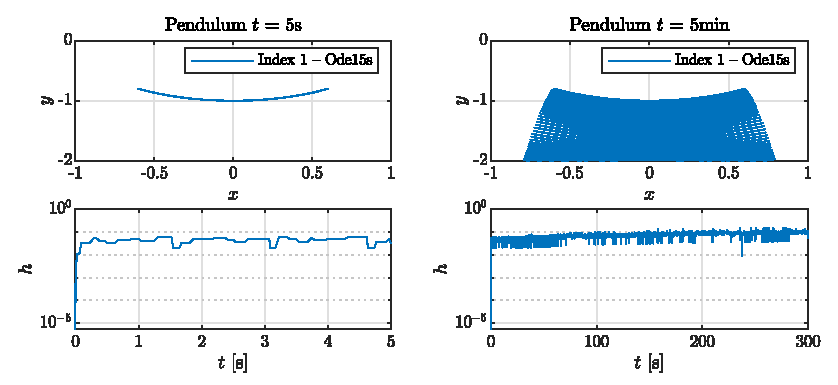
\includegraphics[width=\textwidth]{Figures/Ugf2_14a.eps}
	
	From the above figure it is clear that for a longer simulation time the algebraic constraint given by $e_5$ is no longer satisfied. 
	
	\item[(c)] Better index reduction using  baumgartner stabilization.
	Here, $\ddot e_5$ is replaced with $\ddot e_5 + \alpha\,\dot e_5 + \beta\,e_5$, and $\alpha$, $\beta$ are chosen such that the zeros of $s^2 + \alpha\,s + \beta = 0 $ are to the left half of the $s$-plane. 
	
	For the simulation using  baumgartner stabilization, $\alpha = \beta = 1$. The following figures presents the simulation results:
	
	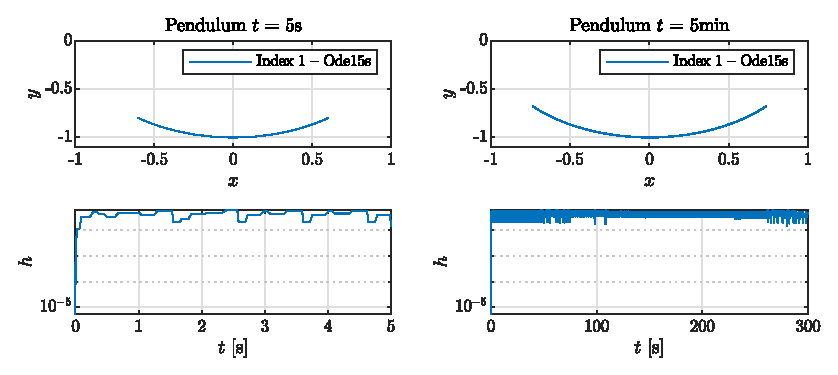
\includegraphics[width=0.9\textwidth]{Figures/Ugf2_14c.eps}
	
	\item[(d)] Add $\epsilon\,\dot \lambda$ on the left-hand-side of the algebraic constraints and simulate using an ODE solver.
	In the model described previously, $e_5$ not becomes as follows:
	\begin{align*}
		\epsilon\,\dot \lambda &= u^2 + v^2 +\lambda\,\frac{x^2 + y^2}{m} - g\,y & \ddot e_5
	\end{align*}
	The matlab solver \texttt{ode45} is unable to meet integration tolerances without reducing the step size below the smallest value allowed (5.551115e-17). The case with $\epsilon=0$ was simulated using \texttt{ode15s}.
	
	Here is the simulation results:
	
	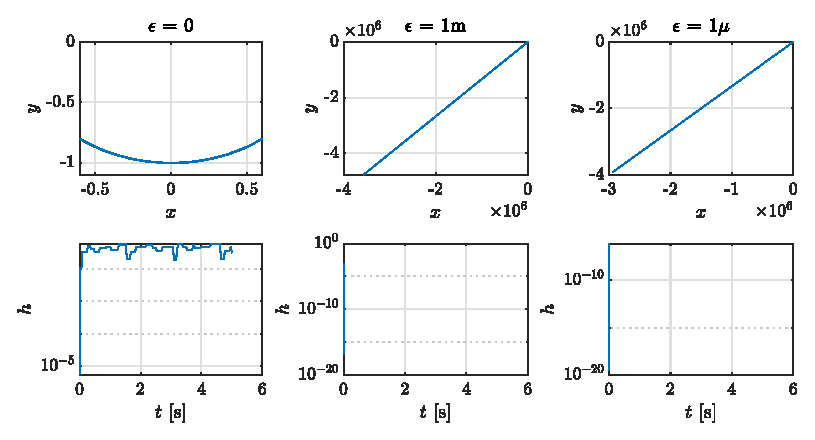
\includegraphics[width=0.55\textheight]{Figures/Ugf2_14d.eps}
	
	Here is the code:
	
	\begin{lstlisting}
		epsilon = [0 1e-3 1e-6]; 
		
		% function definition
		% in pendulam_idx1 y(1) = x, y(2) = y, y(3) = u, y(4) = v, y(5) = lambda
		% lambda from algebraic constraint
		pendulam_idx1_zz = @(t,y) [y(3); y(4); y(5)*y(1); y(5)*y(2) - m*g;
		y(3)^2 + y(4)^2 + y(5)*(y(1)^2 + y(2)^2)/m - g*y(2)]; 
		% Direct index reduction technique
		
		M_idx1_zz = [1 0 0 0 0;
		0 1 0 0 0;
		0 0 m 0 0;
		0 0 0 m 0;
		0 0 0 0 0]; % Mass matrix
		
		M_idx1_zz(end) = epsilon(1);
		options_idx1_zz = odeset('Mass',M_idx1_zz); 
		[t_idx1_l_zz_1,y_idx1_l_zz_1] = ode15s(@(t,y) pendulam_idx1_zz(t,y),tsim_s,y0_idx1,options_idx1_zz);
		
		M_idx1_zz(end) = epsilon(2);
		options_idx1_zz = odeset('Mass',M_idx1_zz); 
		[t_idx1_l_zz_2,y_idx1_l_zz_2] = ode45(@(t,y) pendulam_idx1_zz(t,y),tsim_s,y0_idx1,options_idx1_zz);
		
		M_idx1_zz(end) = epsilon(3);
		options_idx1_zz = odeset('Mass',M_idx1_zz); 
		[t_idx1_l_zz_3,y_idx1_l_zz_3] = ode45(@(t,y) pendulam_idx1_zz(t,y),tsim_s,y0_idx1,options_idx1_zz);
	\end{lstlisting}
\end{enumerate}
	\pagebreak
	\section*{Uppgift 2.15}
	In $\epsilon$-embedding a semi-explicit DAE system makes it closer to an ODE-system. However, as $\epsilon \rightarrow 0$, the mass matrix ($F_{\dot x}$) becomes singular as a result, we can only use implicit solvers. 
	\pagebreak
	\section*{Uppgift 2.18}
	Conservation of invariants. Consider the following model of a chemical reaction:
\begin{align*}
	\dot x_1 &= -0.04\,x_1 + 10^4\,x_2\,x_3,\\
	\dot x_2 &= 0.04\,x_1 - 10^4\,x_2\,x_3 - 3\cdot 10^7\,x_2^2,\\
	\dot x_3 &= 3\cdot 10^7\,x_2^2,
\end{align*}
with the initial conditions:
\begin{align*}
	x_1(0) &= 1, & x_2(0) &= 2\cdot 10^{-4}, & x_3(0) &= 3\cdot10^{-1}
\end{align*}
\begin{enumerate}
	\item[(a)] Show that mass conservation $x_1(t)+x_2(t)+x_3(t) = x_1(0)+x_2(0)+x_3(0) =  M$ is an invariant for the model.
	
	Mass conversation $\implies \dot x_1(t)+\dot x_2(t)+\dot x_3(t) = 0$. \\
	Let the coefficients of $x_1(t),\ x_2(t)\,x_3(t),\ x_2^2(t)$ be $p_1,\ p_2,\ p_3$, respectively. \\
	Then, 
	\begin{align*}
		\dot x_1(t)+\dot x_2(t)+\dot x_3(t) &= -p_1\,x_1 + p_2\, x_2\,x_3 + p_1\,x_1 - p_2\,x_2\,x_3 - p_3\,x_2^2 + p_3\,x_2^2 = 0\\
	\end{align*}
	where, 
	\begin{align*}
		p_1 &= 0.04, & p_2 &= 10^4, & p_3 &= 3\,10^7. 
	\end{align*}*
	Integrating, $\dot x_1(t)+\dot x_2(t)+\dot x_3(t)$, we get: 
	\begin{align*}
		\int \dot x_1(t)+\dot x_2(t)+\dot x_3(t) &= x_1(t) + x_1(0) + x_2(t) + x_2(0) + x_3(t) + x_3(0) = 0\\
		x_1(t) + x_2(t) + x_3(t) &= -(x_1(0) + x_2(0) + x_3(0)) = M
	\end{align*}
	i.e. $x_1(t) + x_2(t) + x_3(t)$ is invariant.
	\item[(b)] The invariant is a linear first integral
	A linear first integral is of teh form:
	\begin{align*}
		c + b^T\,X.
	\end{align*}
	Here,
	\begin{align*}
		X &= [x_1\ x_2\ x_3], & b = []
	\end{align*}
	\item[(c)] Conservation of linear first integrals
	
	The model was simulated in Matlab using \texttt{ode45} RK4-5 solver.
	
	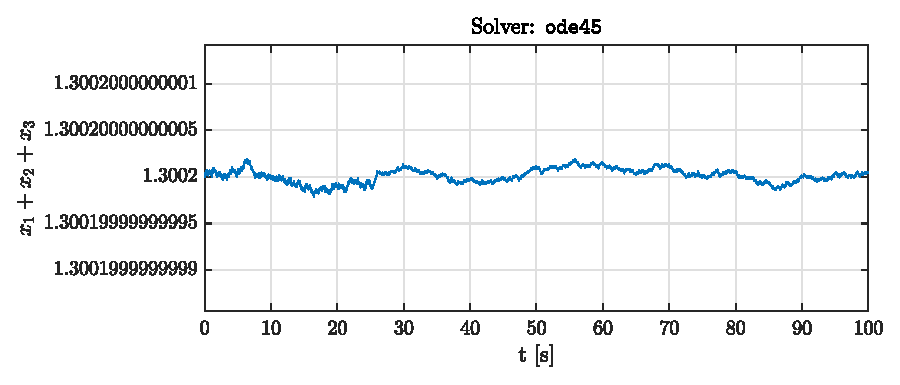
\includegraphics[width=\textwidth]{Figures/Ugf18c.eps}
	
	From the above figure it is clear that the solver  conservers the linear first integral.
	
	\item[(d)] Conservation of quadratic integrals
	The "circle drawer" is given by the following:
	\begin{align*}
		\dot y_1 &= -y_2, & \dot y_2 &= y_1, \\
		y_1(0) &= 1, & y_2(0) &= 0,
	\end{align*}
	The model was simulated in Matlab using \texttt{ode45} RK4-5 solver. The quadratic invariant is given as $y_1^2 + y_2^2$. 
	
	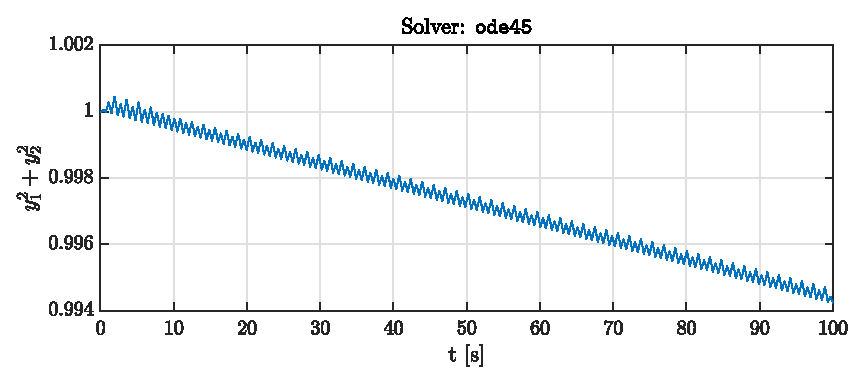
\includegraphics[width=\textwidth]{Figures/Ugf18d.eps}
	
	The above figure presents the quadratic invariant and it is clear that the RK4-5 method does not keep the invariant.
\end{enumerate}
	\pagebreak
	\section*{Uppgift 2.22}
	Jian helped!
\begin{enumerate}
	\item[(a)] \begin{align*}
		 \text{The stabilized system is }\begin{cases}
		 	\dot q &= v \\
		 	m\,\dot v &= f - G^T\,\lambda \\
		 	0 &= \ddot g + \gamma_1\,\dot g + \gamma_2\,g \\		 	
		 \end{cases}
		\end{align*}
	\fbox{\begin{minipage}[h!]{\textwidth}
			$\gamma_1$ and $\gamma_2$ chosen such that the root of the polynomial $s^2 + s\,\gamma_1 + \gamma_2 = 0$ is located in the left-half of the complex plane. 
	\end{minipage}}	
	\item[(b)] \begin{align*}
		\text{Original system: }\begin{cases}
			\dot q &= v \\
			M\,\dot v &= f - G^T\,\lambda \\
			0 &= G\,v = h\\		 	
		\end{cases}
	\end{align*}
	$\dot h + \gamma\,h = 0$ is the stabilization, equivalent to, $G\,\dot v + \frac{\partial G\,v}{\partial q}\,v + \gamma\,G\,v = 0$.
	Therefore, we get:
	\begin{align*}
		\begin{cases}
			\dot q = v \quad & e_1 \\
			M\,\dot v = f - G^T\,\lambda \quad & e_2\\
			G\,\dot v + \frac{\partial G\,v}{\partial q}\,v + \gamma\,G\,v = 0 \quad & e_1\\		 	
		\end{cases}
	\end{align*}
	Focusing on $e_2$:
	Multiply both sides with $G\,M^{-1}$, we get:
	\begin{align*}
		G\,\dot v &= G\,M^{-1}\,f - G\,M^{-1}\,G^T\,\lambda & e_2,\\
		\implies -\frac{\partial G\,v}{\partial q}\,v + \gamma\,G\,v &= G\,M^{-1}\,f - G\,M^{-1}\,G^T\,\lambda & e_2.
	\end{align*}
	Therefore,
	\begin{align*}
		\lambda&= \left(G\,M^{-1}\,G^T\right)^{-1}\,\left(G\,M^{-1}\,f + \frac{\partial G\,v}{\partial q}\,v + \gamma\,G\,v\right)& e_3
	\end{align*}
	substituting $e_3$ in $e_2$, we get:
	\begin{align*}
		\dot v &= M^{-1}\,f - M^{-1}\,G^T\,\left(G\,M^{-1}\,G^T\right)^{-1}\,\left(G\,M^{-1}\,f + \frac{\partial G\,v}{\partial q}\,v + \gamma\,G\,v\right)& e_4
	\end{align*}
	The system equations are:
	\begin{align*}
		\begin{cases}
			\dot q = v \quad & e_1 \\
			\dot v = M^{-1}\,f - M^{-1}\,G^T\,\left(G\,M^{-1}\,G^T\right)^{-1}\,\left(G\,M^{-1}\,f + \frac{\partial G\,v}{\partial q}\,v + \gamma\,G\,v\right) \quad &  e_4 	
		\end{cases}
	\end{align*}
	This is equivalent to:
	\begin{align*}
		\begin{pmatrix}
			\dot q \\
			\dot v 
		\end{pmatrix} &= \hat f(x) - \gamma\,F(x)\,h(x)
	\end{align*}
\end{enumerate}
	\pagebreak
	\section*{Uppgift 2.29}
	The simulation results using Modelica is presented as follows: \\
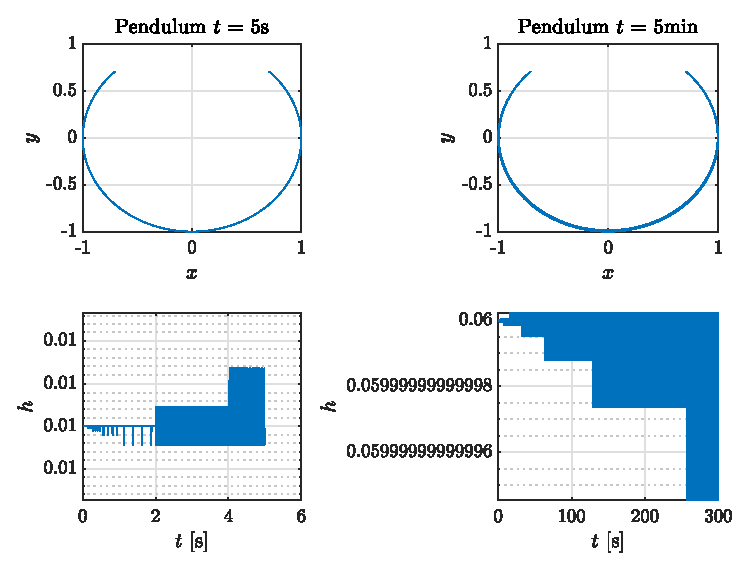
\includegraphics[width=\textwidth]{Figures/Ugf2_29.eps}
The code is as follows:
\begin{lstlisting}
	model Pendulum
		constant pi=3.14
		parameter Real phi0 = 45*pi/180;
		parameter Real L = 1, M = 1, g=9.82;

		Real x(start=L*cos(phi0)), dx(start=0);
		Real y(start=L*sin(phi0)), dy(start=0);
		Real lambda;
	equation
		der(x) = dx;
		der(y) = dy;
		M*der(dx) = lambda*x;
		M*der(dy) = lambda*y-M*g;
		0 = x*x+y*y-L*L;
	end Pendulum;
\end{lstlisting}
	\pagebreak
	\section*{Uppgift 2.30}
	Finding the system of equations to solve to find consistent initial conditions and using the dummy derivatives method to reduce the index to 1. 

The system:
\begin{align*}
	\dot x &= u & e_1\\
	\dot y &= v & e_2\\
	m\,\dot u &= x\,\lambda & e_3\\
	m\,\dot v &= y\,\lambda - m\,g & e_4\\
	0 &= x^2 + y^2 - l^2 & e_5
\end{align*}

Pantelides gives (1,1,0,0,2), i.e:
\begin{align*}
	\ddot x &= \dot u & \dot e_1\\
	\ddot y &= \dot v & \dot e_2\\
	m\,\dot u &= x\,\lambda & e_3\\
	m\,\dot v &= y\,\lambda - m\,g & e_4\\
	0 &= u^2 + v^2 + x\,\ddot x + y\,\ddot y & \ddot e_5
\end{align*}
$\mathcal{G} = (\ddot x,\ddot y,\dot u,\dot v, \lambda)$ can be written as follows:
\begin{align*}
	\begin{tabular}{c|c c c c c}
		& $\ddot x$ & $\ddot y$ & $\dot u$ & $\dot v$ & $\lambda$ \\
		\hline
		$\dot e_1$ & 1 & & 1 & &\\
		$\dot e_2$ & & 1 & & 1 &\\
		$e_3$ & & & $m$ & & $x$\\
		$e_4$ & & & & $m$ & $y$\\
		$\ddot e_5$ & $x$ & $y$ & & &\\	
	\end{tabular} & & \implies & \begin{tabular}{c|c c c c c}
	 & $\ddot x$ & $\ddot y$ & $\dot u$ & $\dot v$ & $\lambda$ \\
	\hline
	$\dot e_1$ & 1 & & 1 & &\\
	$\dot e_2$ & & 1 & & 1 &\\
	$\ddot e_5$ & $x$ & $y$ & & &\\		
\end{tabular}
\end{align*}

\fbox{\begin{minipage}[h!]{\textwidth}
	Assuming $x \neq 0$ then ($\ddot x,\dot u,\dot v$) are chosen as dummy variables. However, $x = 0$ is an equilibrium point of the system. Therefore, ($\ddot y,\dot u,\dot v$) are the chosen dummy variables with the assumption $y \neq 0$. 
\end{minipage}}	

one more dummy variable is required. Therefore, the following equations are considered :
\begin{align*}
	\dot x &= u & e_1\\
	\dot y &= v & e_2\\
	0 &= x\,\dot x + y\,\dot y & \dot e_5
\end{align*}
$\mathcal{G} = (\dot x,\dot y, u)$ can be written as follows:
\begin{align*}
	\begin{tabular}{c|c c c c c}
		& $\dot x$ & $\dot y$ & $ u$ & $ v$ & $\lambda$ \\
		\hline
		$e_1$ & 1 & & 1 & &\\
		$e_2$ & & 1 & & 1 &\\
		$\dot e_5$ & $x$ & $y$ & & &\\		
	\end{tabular} & & \implies & \begin{tabular}{c|c c c c c}
		& $\dot x$ & $\dot y$ & $u$ & $v$ & $\lambda$ \\
		\hline
		$\dot e_5$ & $x$ & $y$ & & &\\		
	\end{tabular}
\end{align*}
\fbox{\begin{minipage}[h!]{\textwidth}
	Since $y \neq 0$ is the assumption, ($\dot  y$) is chosen as the dummy variable. 
\end{minipage}}	
%\begin{description}
%	\item[Assumption 2] Considering $y \neq 0$. 
%\end{description}
%Therefore, we can choose $\dot x$ or $\dot y$ as the dummy variable. $\dot x$ was chosen. \\
%\fbox{\begin{minipage}[h!]{\textwidth}
%	\textbf{Note:} Choosing $\dot x$ would result in a singular matrix when $x = 0$. This is a problem since $x = 0$ is an equilibrium point and the pendulum always passes through this point. 
%\end{minipage}}	

The dummy variables are ($y',y'',u',v'$). 

The equation set with variables $(x,y,y',y'',u,v,u',v',\lambda)$ is given as follows:
\begin{align*}
	\dot x &= u & e_1\\
	\dot u &= u' & \dot e_1\\
	y' &= v & e_2\\
	y'' &= v' & \dot e_2\\
	m\,u' &= x\,\lambda & e_3\\
	m\,v' &= y\,\lambda - m\,g & e_4\\
	0 &= x^2 + y^2 - l^2 & e_5\\
	0 &= x\,u'+ y\,y' & \dot e_5 \\
	0 &= u^2 + v^2 + x\,u' + y\,y'' & \ddot e_5
\end{align*}
The simulation results are presented in the following figure:\\
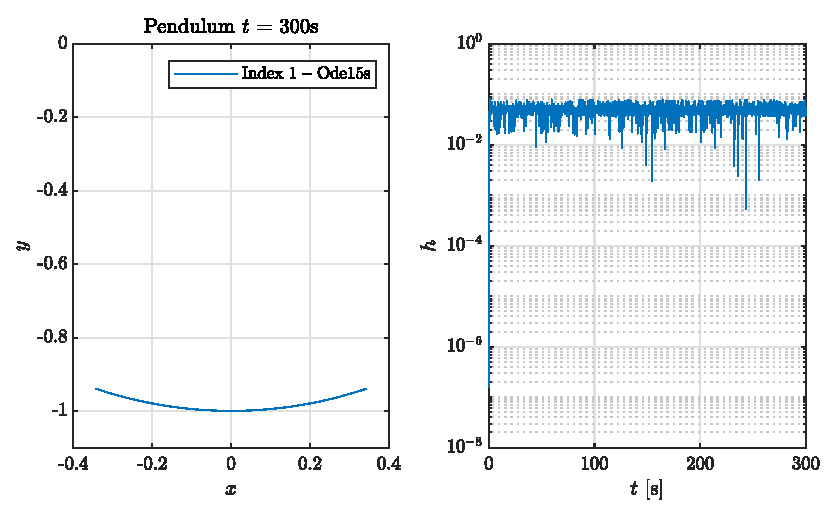
\includegraphics[width=0.9\textwidth]{Figures/Ugf2_30.eps}

The code is as follows:
\begin{lstlisting}
	clear all; clc; 
	% the DAE system for the pendulum
	% parameters
	m = 2.6; % mass of the pendulam
	g = 9.8; 
	l = 1; % length of the pendulam
	
	% The Model
	% y(1) = x
	% y(2) = u
	% y(3) = y'
	% y(4) = y''
	% y(5) = y
	% y(6) = v
	% y(7) = u'
	% y(8) = v'
	% y(9) = lambda
	pendulam_idx1 = @(t,y) [ ...
	y(2);...
	y(7);...
	y(6) - y(3);...
	y(8) - y(4);...
	y(1)*y(9) - m*y(7);...
	y(5)*y(9) - m*g - m*y(8);...
	y(1)^2 + y(5)^2 - l^2;...
	- y(5)*y(3);...
	y(2)^2 + y(6)^2 + y(1)*y(7) + y(5)*y(4)]; 
	% simulation 
	tsim_l = [0 300]; % long simulation time
	
	M_idx1 = zeros(9,9); % mass matrix
	M_idx1(1,1) = 1; M_idx1(2,2) = 1; 
	options_idx1 = odeset('Mass',M_idx1); 
	
	y0 = -l; y0_idx0 = [0;1;0;0;y0;0;0;0;0]; % initial conditions
	
	[t_idx1_l,y_idx1_l] = ode15s(@(t,y) pendulam_idx1(t,y),tsim_l,...
	y0_idx0,options_idx1);
	
	% Plots
	figure(1)
	clf
	
	subplot(121)
	plot(t_idx1_l(:,1),y_idx1_l(:,5)) %,y_idx0_s(:,1),y_idx0_s(:,2),'--')
	grid on; legend('Index 1 -- Ode15s') %,'Index 0 -- Ode45')
	ax(1) = figtex(gca,1);
	xlabel('$x$'); ylabel('$y$'); title('Pendulum $t$ = 300s');
	ylim([-l*1.1 0])
	
	subplot(122)
	semilogy(t_idx1_l(2:end),diff(t_idx1_l)) %,t_idx0_s(2:end),diff(t_idx0_s),'--')
	grid on; ax(3) = figtex(gca);
	xlabel('$t$ [s]'); ylabel('$h$');
	
	figsize(1,0.35);
	saveas(gcf,'Figures/Ugf2_30','epsc');		
\end{lstlisting}
	\pagebreak
	\section*{Uppgift 2.31}
	The initial ODE initial value problem:
\begin{align*}
	\dot y + y\,\theta &= 0, & y(0) &= y_0.	
\end{align*}
The  performance measure is given as follows:
\begin{align*}
	G = \int_{0}^{T}y^2(t)\,dt
\end{align*}
Computing $dG/d\theta$ with $T = 5,\ \theta=1$ and $y_0 = 2$.
\begin{enumerate}
	\item[(a)] Exact, analytical, expression
	
	The analytical solution to the ode is $y = y_0\,e^{-t\,\theta}$.
	Now, $$\frac{dG}{dt}\Bigg|_{T = 5,\ \theta = 1} = \textbf{-1.9990}$$
	\item[(b)] Forward sensitivity analysis
	The implementation of the Forward sensitivity analysis in Matlab is presented as follows:
	\begin{align*}
		\dot y & = -y\,\theta, \text{ is of the form}\ \dot X = f(t,X,p), \text{then:} \\
		f_x &= -\theta, \\
		f_p &= -y \\
		X_p &= -\theta\,y_0\,e^{-\theta\,t} \\
	\end{align*}
	Now we solve the follows ODEs:
	\begin{align*}
		\dot y & = -y\,\theta\ \& &\  \dot X_p &= f_x\,X_p + f_p & \frac{dG}{dP} &= 2\,X_p\,y
	\end{align*}
	From this we get $$\frac{dG}{dt}\Bigg|_{T = 5,\ \theta = 1} = \textbf{-1.9998}$$
	The simulations results are presented in the followsing figure:
	
	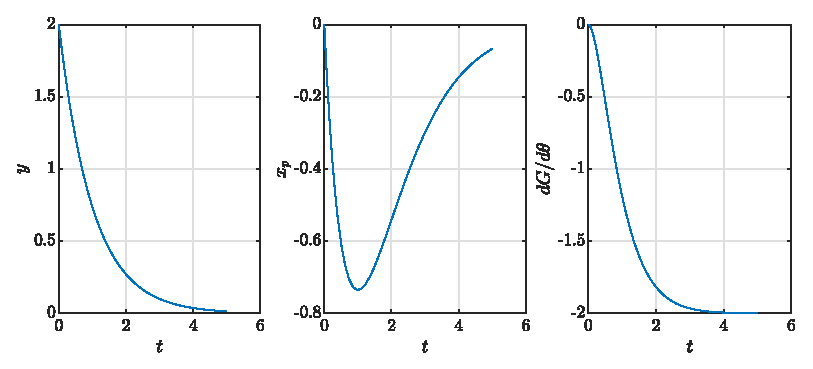
\includegraphics[width=0.9\textwidth]{Figures/Ugf21b.eps}
	
	The code implementation in Matlab is as follows:
	\begin{lstlisting}
		y0 = [2, 0, 0]; theta = 1;
		
		f = @(t,y) [-theta*y(1); ... y
		-theta*y(2) - y(1);... Xp
		2*y(1)*y(2)... dG/dp
		]; 
		
		options = odeset('RelTol',RelTol,'AbsTol',AbsTol); % setting finer tolerences
		[t,yval] = ode45(@(t,y) f(t,y),[0 5],y0);
	\end{lstlisting}
	\item[(c)] Adjoint sensitivity analysis
	
	The implementation of the Adjoint sensitivity analysis in Matlab is presented as follows:
	\begin{align*}
		\text{let, }F &= \dot y + \theta\,y,\ & g&= y^2, \text{ then,}\\
		F_x &= \theta\ \&\ \dot F_x = 1, & g_x &= 2\,y		
	\end{align*}
	Now, we need to solve for $\lambda$ backwards from $T$
	\begin{align*}
		(-\lambda\,\dot F_x)' + \lambda\,F_x + g_x &= 0,
	\end{align*}
	Here we define the following:
	\begin{align*}
		z(\tau) &= x\,(T - \tau),\ t = T - \tau;\ \text{where,}\\
		\dot x &= -y(T -t) = -\dot y(\tau), & x(t) &= y(T-\tau) = y(\tau),\ \text{and,}\\
		-y(\tau) &= -\lambda(T-\tau), & y(\tau) &= \theta\,\lambda(T-\tau),\ \text{and,}\\
		g_x &= 2\,y(t-\tau).
	\end{align*}
	Using $\lambda$, we calculate $\frac{dG}{d\theta}$ using the following relation:
	\begin{align*}
		\frac{dG}{d\theta} &= \int g_p - \lambda(t)\,F_p dt,\text{ where}
		g_p &= -\theta\,y, & F_p &= y
	\end{align*}
	Thus, we get $$\frac{dG}{dt}\Bigg|_{T = 5,\ \theta = 1} = \textbf{-1.9856}$$
	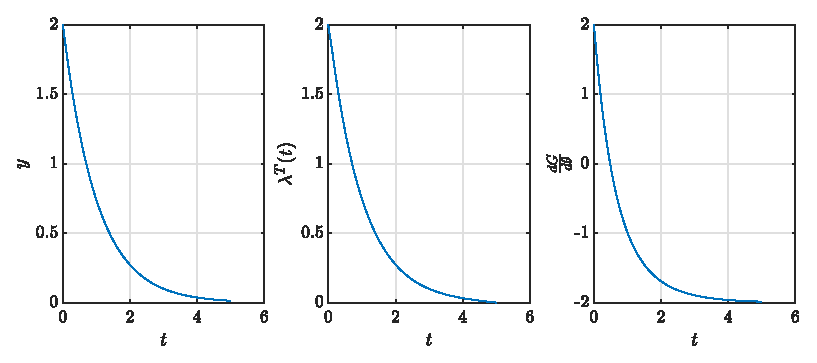
\includegraphics[width=\textwidth]{Figures/Ugf31c.eps}
	The code is presented as follows:
	\begin{lstlisting}
		T = 5; % final time 
		theta = 1; y0 = 2;
		
		f1 = @(t,y) -theta*y; ... y
		
		options = odeset('RelTol',RelTol,'AbsTol',AbsTol); % TOL setting
		[tsim,yval_2] = ode45(@(t,y) f1(t,y),[0 5],y0,options); % solving for y
		
		gx = @(t) interp1(tsim,2*yval_2,t,'spline'); % 2*y(tau) //ERROR should be Tau not t
		f2 = @(tau,lambda) -theta*lambda + gx(T - tau); % DE for lambda
		
		lambda_fin = 0; % initital guess based on lambda*Fx' = 0; since Fx' is 1, lambda = 0.
		[tsim_lambda,lambda_val] = ode45(@(t,y) f2(t,y),[0 5],lambda_fin,options); % solving for lambda
		
		tsim_lambda_t = flipud(T - tsim_lambda);
		lambda_t = flipud(lambda_val)'; % flipping the lambda and making it w.r.t t

		x0 = 1*theta*lambda_t(1);% Fx'(0)*Fx(0)*lambda(0)
		
		f3 = @(t,x) -theta*interp1(tsim,yval_2,t,'linear') - interp1(tsim_lambda_t,lambda_t,t,'spline')*interp1(tsim,yval_2,t,'linear'); % dG/dp
		[tsim_dGdp,dGdp_val] = ode45(@(t,y) f3(t,y),[0 5],x0,options); % just integrating
	\end{lstlisting}
\end{enumerate}
The following table presents $\frac{dG}{dt}|_{T = 5,\ \theta = 1}$ using all the three methods of sensitivity analysis.
\begin{center}
	\begin{tabular}{c|c|c}
		Analytical & Forward & Adjoint \\
		\hline
		-1.9990 & -1.9998 & -1.9856
	\end{tabular}
\end{center}

	\pagebreak
	\section*{Uppgift 2.33}
	\textit{DAE simulation functionality in Matlab}

The simulation of the chemical reactions are presented as follows:

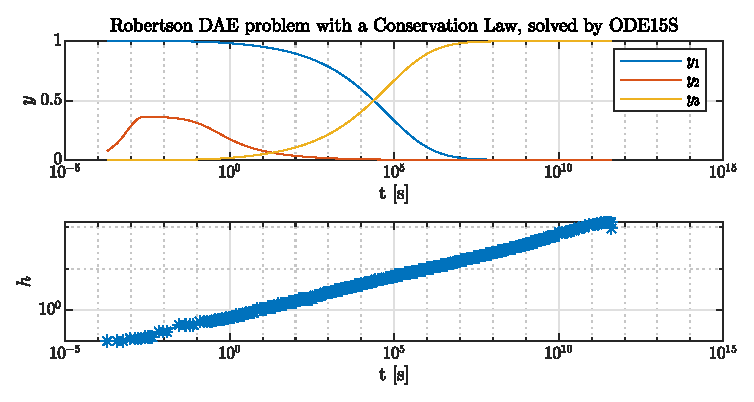
\includegraphics[width=\textwidth]{Figures/Ugf233.eps}

The code is given as follows:

\begin{lstlisting}
	clc; clear all;
	
	p1 = 0.04; p2 = 10e4; p3 = 3e7; % Constants 
	y0 = [1; 0; 0]; % initial conditions
	
	% function definition
	robertsdae = @(t,y) [-p1*y(1) + p2*y(2).*y(3); 
	p1*y(1) - p2*y(2).*y(3) - p3*y(2).^2;
	y(1) + y(2) + y(3) - 1 ];
	
	% simulation
	tsim = [0 40e10]; % simulation time
	M = [1 0 0; 0 1 0; 0 0 0]; % Mass matrix
	options = odeset('Mass',M);
	% play with the tols and try with ode15i
	
	[t,y] = ode15s(@(t,y) robertsdae(t,y),tsim,y0,options);
\end{lstlisting}

It is worth mentioning that the initial conditions are computed internally when we use the \texttt{ode15s} solver. However, another approach is to use the implicit solver \texttt{ode15i} and the initial conditions are given by using the function \texttt{decic}.
	\pagebreak
	
\end{document}